\documentclass[twoside]{article}
\usepackage{ecj,palatino,epsfig,latexsym,natbib}
\usepackage{float} % lets you have non-floating floats
\usepackage{url} % for typesetting urls
\usepackage{graphicx} % for including images
\usepackage{caption}
\usepackage{program}
\usepackage{tabularx}
\usepackage{colortbl}
\usepackage{algorithm, algpseudocode}

\usepackage{amsmath,amssymb}
%\usepackage{mathtools}
\usepackage{etoolbox}
\usepackage{hhline}
\usepackage{subcaption}
\newfloat{fig}{thp}{lof}[section]
\floatname{fig}{Figure}
\let\bbordermatrix\bordermatrix
\patchcmd{\bbordermatrix}{8.75}{4.75}{}{}
\patchcmd{\bbordermatrix}{\left(}{\left[}{}{}
\patchcmd{\bbordermatrix}{\right)}{\right]}{}{}

\makeatletter
\def\BState{\State\hskip-\ALG@thistlm}
\makeatother



%% do not add any other page- or text-size instruction here

\parskip=0.00in

\begin{document}

\ecjHeader{x}{x}{xxx-xxx}{201X}{45-character paper description goes here}{Tan, Ma, Zhang}
\title{\bf Optimization of Location Allocation of Web Service using non-dominated sorting algorithm(NSGA-II)
}  

\author{\name{\bf Boxiong Tan} \hfill \addr{tanboxi@ecs.vuw.ac.nz}\\ 
        \addr{Department of Science and Engineering, Victoria of Wellington, 
        Wellington, Zip, New Zealand}
\AND
       \name{\bf Hui Ma} \hfill \addr{hui.ma@ecs.vuw.ac.nz}\\
        \addr{Department of Science and Engineering, Victoria of Wellington, 
		Wellington, Zip, New Zealand}
}

\maketitle

\begin{abstract}

The abstract goes here.  It should be about 200 words and give the
reader a summary of the main contributions of the paper.   
Remember that readers may decide to read or not to read your
paper based on what is in the abstract.  The abstract never
contains references.  

\end{abstract}

\begin{keywords}

multi-objective,
NSGA-II,
genetic algorithms, 
evolutionary programming

\end{keywords}
\section{Introduction}
Web Services are considered as self-contained, self-describing, modular applications that can be published, located, and invoked across the Web \cite{Ran:2003:MWS:844357.844360}. 
In recent years, web services technology is becoming increasingly popular because the convenience, low cost and capacity to be composed into high-level business processes \cite{Aboolian200964}.
Because of modularization and open interfaces, Web services facilitate the development of highly 
customizable and adaptable applications to meet business demand. Furthermore, Web services offer a 
convenient registration, search  and discovery system. e.g. Universal Description, Discovery and Integration (UDDI). 

With the ever increasing number of functional similar web services being available on the Internet, the web service providers (WSPs) are trying to improve the quality of service (QoS) to become competitive in the market.  
QoS also known as non-functional requirements to  web services, is the degree to which a service meets specified requirements or user needs \cite{4061431}, such as response time, security and availability. 
Among numerous QoS measurements, service response time is a critical factor for many real-time services, e.g. traffic service or finance service. 
Service response time has two components: transmission time (variable with message size) and network latency \cite{Johansson:2000:INL:595252.595281}. 
Study \cite{916684} has shown that network latency is a significant component of service response delay.
Ignoring network latency will underestimate response time by more than 80 percent. Since network latency is related to network topology as well as physical distance \cite{distanceMetrics}. 
The network latency could also vary with the network topology changes.
The only way to reduce the network latency is move the service to a location where has smaller network latency to the user center. 
Hence, the WSPs need to consider which physical location to deploy their services so that it could minimize the cost as well as ensure the QoS.

The Web service location-allocation problem is essentially a multi-objective optimization problem \cite{Multiobjective}.
Because of the confliction between service quality and deployment cost. 
Ideally, WSP could deploy their services to each user center in order to provide the best quality.
That is, the more services deployed, the better the quality and the higher cost. 
This problem is considered as an NP-hard due to the fact that the combinatorial explosion of the search space \cite{Vanrompay:2008:GAO:1387309.1387313}. 


Very few researches \cite{Aboolian200964, Sun} study this problem.
Both studies try to solve the problem by integer linear programming techniques.
In particular, \cite{Sun} has solved this problem by employ a modified Alternate Location-Allocation (ALA) algorithm. 
However, essentially ALA build upon integer programming and use greedy algorithm to optimize the result. 
As a result, the solution is easily stuck at local optima.

Evolutionary algorithms (EAs) have been used in solving multi objective optimization problems in recent years. 
EAs are ideal for solving multi objective optimization problems \cite{key:article}, since EA works with a population of solutions, 
a simple EA can be extended to maintain a diverse set of solutions.
With an emphasis for moving toward the true Pareto-optimal region, an EA can be used to find multiple Pareto-optimal solutions in one single simulation run \cite{OptimizationElectrical}.

Hai \cite{EnhancedGenetic} proposed an enhanced genetic algorithm-based approach which make use of the integer scalarization technique to solve the multi-objective problem.
The genetic algorithm (GA) is an EA that uses genetic operators to obtain optimal solutions without any assumptions about the search space.
This algorithm solve the scalability problem in the dataset, however the integer scalarization technique \cite{Multiobjective} has some disadvantages: 

\begin{enumerate}
	\item The decision maker needs to choose an appropriate weights for the objectives to retrieve a satisfactorily solution.
	\item The algorithm does not produce an uniform spread of points on the Pareto curve. That is, all points are grouped in certain parts of the Pareto front.
	\item Non-convex parts of the Pareto set cannot be reached by minimizing convex combinations of the object functions.
\end{enumerate}

Evolutionary multi objective optimization (EMO) methodologies on the other hand, successfully avoid the above mentioned problems and demonstrated their usefulness in find a well-distributed set of near Pareto optimal solutions \cite{Aboolian200964}. Non-dominated sorting GA (NSGA-II) \cite{996017}, Strength Pareto Evolutionary Algorithm 2 (SPEA-2) \cite{Deb:2005:EED:1109044.1109049} have become standard approaches. 
Some schemes based on particle swarm optimization approaches \cite{Elhossini:2010:SPP:1739146.1739151, Huang:2006:CLP:1108677.1108683} are also important. 
Among numerous EA approaches, NSGA-II is one of the most widely used methods for generating the Pareto frontier. 
NSGA-II implements elitism and uses a phenotype crowd comparison operator that keeps diversity without specifying any additional parameters \cite{Deb06referencepoint}.
In our approach, we apply a modified version of NSGA-II since the web service location-allocation is a discrete problem. 

The main purpose of this research is to provide a framework that guides a WSP to locate its servers.
We consider the problem faced by a WSP who has existing facilities but wishes to use the collected data to re-allocate their services in order to maximum their profit.
The WSP must decide on facility locations from a finite set of possible locations. 
In order to make the decision, the WSP must first analyze the data which were collected from current services. 
The collected data should includes the records of invocation from each unique IP address.
Therefore, based on these data, the WSP could summarize several customer demand concentrated at \textit{n} discrete nodes \cite{Aboolian200964}, namely user centers. 
We assume the WSP has already done this step and list of user centers and candidate service deployment locations are given.
In addition to decide which location to re-allocate the services, a dataset which contains the network latency between demand user center and candidate location are critical. 
The WSP could collect the data or use existed dataset \cite{5552800, 6076756}. 
Then, the service provider could use the algorithm which proposed by this paper, to select an optimal plan based on their funds. 
The algorithm will produce a near optimal solution which indicate the services deployment locations with a minimum cost and best service quality.
The main objectives are:
\begin{itemize}
	\item To model the web service location-allocation problem so that it can be tackled with NSGA-II
	\item To develop a modified NSGA-II approach for the web service location-allocation problem
	\item To evaluate our approach by comparing it to a GA approach which use integer scalarization technique.
\end{itemize}


In Section 2 we provide a formulation for our model. Section 3 develops a modified NSGA-II. 
We use these to study a number of hypotheses on the placement of WSPs. These solutions are compared to solutions from ALA. 
The experiments and their result are discussed in Section 4. We end with a discussion of our results and possible future 
research directions in Section 5.








\section{Problem Description}
\subsection{Model formulation}
The problem is to determine which facility locations that could maximus WSPs’ profit 
as well as ensure low network latency. 
Let $S = \{ 1, 2, ..., s\}$ be the set of services. We assume that the demand for service is concentrated at $i$ 
demand nodes $I = \{ 1, 2, ..., i \}$. Let $J = \{ 1, 2, ..., j \}$ be the set of $j$ candidate facility locations.
To model the service location-allocation problem we use four matrices: service network latency matrix $L$, service location
matrix $A$, service invocation frequency matrix $F$ and cost matrix $C$.

The server network latency matrix $L = [l_{ij}]$, is used to record network latency from user centers to 
candidate locations, where $l_{ij}$ is a real number denotes the network latency from user center $i$ to candidate 
location $j$. 
These data could be retrieved from implementing a network latency experiment or using existed datasets \cite{5552800, 6076756}.
\begin{center}
$
L = \bbordermatrix{~ & j_{1} & j_{2} & j_{3} \cr
					i_{1}	&0 &5.776 &6.984	\cr
					i_{2}	&5.776  &0 &2.035 \cr
					i_{3}	&0.984 &1.135	&2.3 \cr} 
$
\end{center}
The service location matrix $A = [y_{sj}]$ represents the actual service location-allocation, where $y_{sj}$  is a binary value ( i.e., 1 or 0) shows whether a service $s$ is deployed in candidate location $j$ or not.
We use the service location matrix A as the representation of chromosome that evolve itself during the progress.
\begin{center}
$
A = \bbordermatrix{~ & j_{1} & j_{2} & j_{3}\cr
					s_{1}	&0 &1 &0	\cr
					s_{2}	&0  &0 &1	\cr
					s_{3}	&1 &1 &0	\cr} 
$
\end{center}

The service invocation frequency matrix $F= [f_{is}]$, is used to record services invocation frequency from user centers, which $f_{is}$ is an integer that indicate the number of invocation in a period of time from user center $i$ to service s. e.g. 120 invocations per day from user center $i_{1}$ to $s_{1}$.
\begin{center}
$
F = \bbordermatrix{~ & s_{1} & s_{2} & s_{3}  \cr
					i_{1}	&120 &35 &56	\cr
					i_{2}	&14  &67 &24 \cr
					i_{3}	&85 &25 &74 \cr} 
$
\end{center}

The cost matrix $C = [c_{sj}]$, is used to record the cost of deployment of services from candidate locations, 
which $c_{sj}$ is an integer that indicate the cost of the deployment fee from a candidate location. 
e.g 130 \$ to deploy $s_{1}$ from $j_{1}$.
\begin{center}
$
C = \bbordermatrix{~ & j_{1} & j_{2} & j_{3}\cr
					s_{1}	&130 &80 &60\cr
					s_{2}	&96  &52 &86\cr
					s_{3}	&37 &25 &54\cr} 
$
\end{center}

Consider the following key modeling assumptions:
\begin{enumerate}
	\item The new WSP decides where to locate his facilities regardless if there is existed functional similar services from other WSPs.
	\item This choice is made only consider two factors: total network latency and total cost.
	\item We assume a fixed customer allocation policy for WSPs. In practice, Web Services typically offer clients persistent and interactive services, which often span over multiple sessions. Therefore, a dynamic reallocation scheme is not practical as it may disrupt the continuity of the services.
\end{enumerate}

\section{Modified NSGA-2 algorithm}
NSGA-2 belong to the larger class of evolutionary algorithms (EAs), which generate approximate solutions to 
optimization and search problems by using techniques inspired by the principles of natural 
evolution: selection, crossover and mutation.

\begin{algorithm}
	\caption{modified NSGA-2 algorithm}
	\label{NSGA2}
	\begin{algorithmic}[1]
		\State Initialize a population of chromosome with random binary value
		\State Evaluate with fitness functions
		\State Non-dominated sort and assign ranking to each chromosome
		\State Evaluate the Crowding distance of each chromosome
		\State Initialize the Pareto Front Pool
		\While{predefined generation}
		\State Tournament Selection
		\State Crossover 
		\State Mutation
		\State Constraint Check and repair operation
		\For(each chromosome)
		\If{chromosome does not exist in the Pareto front Pool}
		\State Evaluate with fitness functions
		\EndIf
		\State Non-dominated sort and assign ranking
		\State Evaluate the Crowding distance
		\EndFor
		\State Recombination and Selection
		\State Pareto Front Pool $\leftarrow$ Current Pareto Front
		\EndWhile
	\end{algorithmic}
\end{algorithm}

There are two major differences between standard NSGA-II and modified version. Firstly, in order to avoid repeat evaluation of the Fitness
of chromosome which contribute to the majority of computation. After the first generation is initialized, the Pareto front will be 
stored in the memory. In each generation, when evaluate the chromosome, the chromosome will be check whether it is existed in the memory pool. 
If so, then the calculation of fitness will be skipped. At the end of each iteration, the Pareto front will be replaced by the latest front.
The reason for setting a memory pool is that, after a number of iteration, the population start converging. 
Most of the population are redundant. Therefore, a memory pool could considerably reduce the repeat computation.

The order major difference is the genetic operators which was discussed in \ref{sec:operators}.

\subsection{Chromosome Representation}
In our problem, the chromosome is the service location matrix A that we mentioned in the previous section. 
\subsection{Objectives and Fitness Function}
The objective functions of this entire problem are following:
\begin{itemize}
	\item Minimize the total cost of services. n is the number of service, m is the number of candidate location.
		\begin{center}
			\begin{equation}
				CostFitness = \sum\limits_{s \in S} \sum\limits_{j \in J} C_{sj} \times A_{sj}
			\end{equation}
		\end{center}
	\item Minimize the network total latency of the services. There are some assumptions we made of network latency. First, we assume
			the latency = 0 if the service is deployed locally. That is, if the service is deployed in the user center A. Then, the 
			invocation from A to the service will be 0 latency. The second assumption is the latency is symmetrical between cities. e.g. 
			The latency from city A to city B is same with the latency from city B to city A. Thirdly, the total invocation are equally
			contribute by user centers.
		\begin{itemize}
			\item For each chromosome, firstly, calculate the number of invocation for each service.
				\begin{center}
					$Invocation_{s} = \sum\limits_{i \in I} F_{is}$
				\end{center}
			\item Calculate the total number of each services.
				\begin{center}
					$ServiceNo_{s} = \sum\limits_{s \in S}\sum\limits_{j \in J} A_{sj}$
				\end{center}
			\item Calculate the number of each service deployed in each location.
				\begin{center}
					$ServiceNo_{sj} = \sum\limits_{j \in J} A_{sj}$
				\end{center}
			\item Calculate the average number of each user center contribute to the total number of invocation of each services.
				\begin{center}
					$AverageInvocation_{i} = Invocation_{s} \div ServiceNo_{s} \div ServiceNo_{sj}$
				\end{center}

			\item Calculate the latency of each service by multiply latency matrix $L$ by service allocation matrix $A$(chromosome).
				\begin{center}
					$LocationLatency_{i} = \sum\limits_{i \in I} L_{ij} \times A_{sj}$
				\end{center}

			\item Calculate the total latency of the multiplication of $AverageInvocation_{i}$ and $LocationLatency_{i}$.
				If the service is deployed locally, then the latency equals zero.
				\begin{center}
						Check if deployed locally: $LocationLatency_{i}$ = 0
				\begin{equation}
						LatencyFitness = \sum\limits_{s \in S}\sum\limits_{i \in I} AverageInvocation_{i} \times LocationLatency_{i}
				\end{equation}
				\end{center}
		\end{itemize}
\end{itemize}
The population is initialized based on the problem range and constraints. 
In our problem, we have two constraints, the cost constraint and minimum number of service constraint. 
If the initialized chromosome does not satisfy the constraints, then repair operators will attempt to 
recover from possible constraint violations. The detail of repair operators will be discuss in next section.
\subsection{Constraints}
The our approach, each chromosome have to satisfy two constraints to be a feasible solution.
The first constraint controls the service number which is make sure that each service is deployed in at 
least one location.
\begin{center}
	\begin{equation}
		\sum\limits_{s \in S} A_{sj} \geq 1
	\end{equation}
\end{center}

The second constraint is cost constraint which predefined the upper boundary of the total cost.
An integer number CostLimitation is defined. This constraint will try to constraints
\begin{center}
	\begin{equation}
		\sum\limits_{s \in S} \sum\limits_{j \in J} C_{sj} \times A_{sj} \leq CostLimitation
	\end{equation}
\end{center}
The constraint is implemented by repair operators which is introduced in the next section.

\subsection{Genetic operators}
\label{sec:operators}
Specific selection, mutation and crossover operators were implemented. It is important to note that mutation and 
crossover operators can produce solutions that might violate the constraints. Therefore, repair 
operators are needed to try to maintain feasible solutions. The original NSGA-II use a simulated 
binary crossover (SBX) \cite{930314} and polynomial mutation \cite{Raghuwanshi04} to cope with continuous problem. 
However, our problem is discretized, therefore we use the regular GA mutation and crossover.


\subsubsection{Mutation}
The mutation operator works as follows: Initially choose one random location from the chromosome. 
Then, reverse the bit, e.g. 0 to 1 or 1 to 0. 

In this study, a chromosome in a population will be selected based on mutation possibility $P_{m}$. 
As shown in below, a random position will be selected and replaced by a reversed number.
\begin{figure}[ht]
\centering
	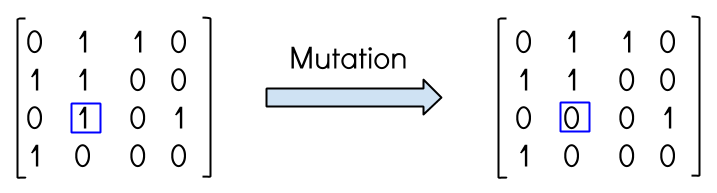
\includegraphics[width=0.5\textwidth]{pics/mutation.png}
\caption{}
\label{graph1}
\end{figure}
\subsubsection{Crossover}
The crossover operator in this paper is the single point crossover. 
The crossover is controlled by crossover probability $P_{c}$. 
The crossover point is created randomly within the length of the chromosome. 
As in the example below, two parents crossover at a point, then two offspring were generated.
\begin{figure}[ht]
\centering
	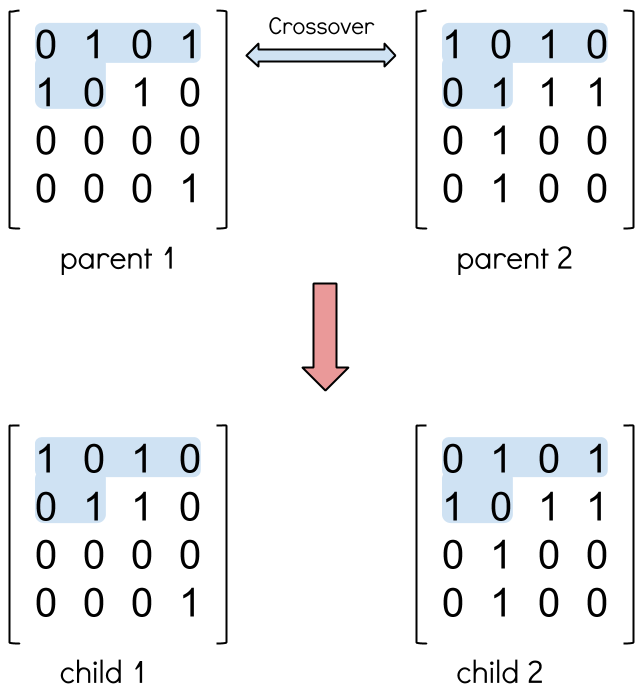
\includegraphics[width=0.3\textwidth]{pics/crossover.png}
\caption{}
\label{graph1}
\end{figure}


\subsubsection{Repair operators}
Since mutation and crossover are very likely to generate offspring that violate the constraints, therefore, 
repair operators are necessary. Normally, each constraint would has an unique repair operator 
in order to recover different types of violation.

After the process of mutation and crossover, the repair operators are examine each chromosome. 
If there is violation found in the chromosome, then it will try to repair it. 
In our problem, we have two repair operators: service number and cost.

\begin{flushleft}\textbf{Service number repair operator}\end{flushleft}
\begin{center}
		$\sum\limits_{s \in S} A_{sj} \geq 1$ \\
		service number constraint
\end{center}
The operator will go through each row of the Location Allocation matrix A, if the number of each 
service is less than one, then randomly choose one location and reverse the selected bit. 
Although the randomness does not necessarily provide an optimal solution, the computation time is 
better than exhaustively compare all solutions. 


\begin{flushleft}\textbf{Cost repair operator}\end{flushleft}
	\begin{center} 
		$\sum\limits_{s \in S} \sum\limits_{j \in J} C_{sj} \times A_{sj} \leq CostLimitation$ \\
		cost constraint
\end{center}

If the cost exceed the predefined limitation. Then the operator would iteratively check if any service has 
been deployed in more than one location. After found one service has been deployed multiple locations, 
the operator will randomly select one of them and change to zero. That means, cancel the deployment of 
that service in this location. After doing that, re-examine the chromosome, if it is still exceed the 
limitation then repeat this process until there is no redundant services or it satisfies the constraint.

This algorithm will try its best to reduce the cost regardless of other factors. Although the modified 
chromosome may end up with higher network latency, however the cost constraint has higher priority than network latency.

Worth noting that this algorithm may not provide a strictly correct solution that satisfied the constraint, 
partially because the randomly chosen of canceling deployment. On the other hand, it may also indicate that 
the predefined upper boundary of cost limitation is too low.

\section{Experiment Design}
The purpose of the experiment is comparison between Alternate Location Allocation (ALA) with modified NSGA-II in terms of efficiency and quality of solutions. 

The exact algorithm was coded in R using packages: NSGA2R and LpSolve. The program was run on a 3.40GHz 
desktop computer with 8 GB RAM.

To compare with ALA, four different datasets were used, the problem instance was generated as follows:
\begin{enumerate}
	\item The potential user center and candidate nodes were randomly selected from existed network latency dataset. 
	\item The number of potential user center equals the candidate nodes. We defined 4 different size of allocation matrices:
			$3 \times 3, 5 \times 5, 10 \times 10$ and $15 \times 15$.
	\item Network latency $L_{ij}$ were selected from network latency dataset based on the user centers and candidate nodes that
		we chose previously.
	\item The cost matrix was randomly generate from a normal distribution which mean = 100 and standard deviation = 20
	\item The frequency matrix was an integer matrix which randomly generate from a uniform distribution on [1, 120]
\end{enumerate}

In each dataset, algorithms run under four different level of cost constraint: Sufficient condition is 100\% the expected total cost, 
good condition (80\%), pool condition (40\%) and minimum budget condition (0\%). The NSGA-II runs 40 times with different random 
seed ranging from 1 to 40. In efficiency test, We evaluate the average run time for each algorithm. 

In order to compare the solution set from  NSGA-II and a single solution from ALA, we employ non-dominated Pareto front
\cite{Xue:2012:MPS:2330163.2330175} and Dominance Relation \cite{1688438}.
40 results (from 40 runs) under each cost constraint are presented in the Section \ref{sec:comparison}. 40 sets of solutions 
achieved by each multi-objective algorithm are firstly combined into one union set. In the union set, the non-dominated solutions 
are presented to compare with the solutions achieved by ALA.

\begin{figure}[H]
	\centering
	\begin{subfigure}[b]{0.4\textwidth}
		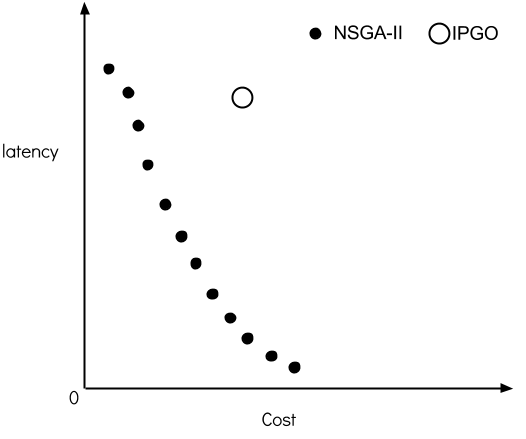
\includegraphics[width=\textwidth]{pics/1.png}
		\caption{}
	\end{subfigure}%
	\begin{subfigure}[b]{0.4\textwidth}
		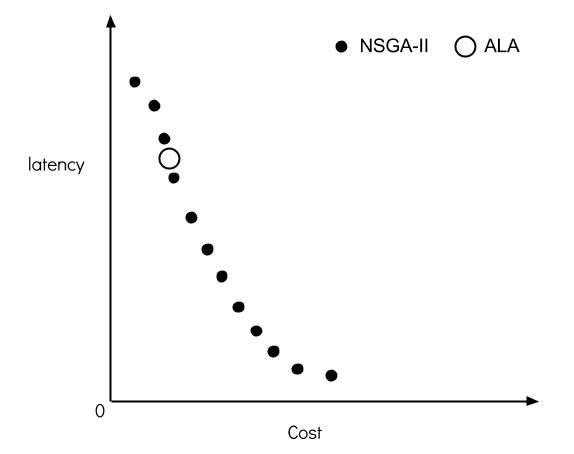
\includegraphics[width=\textwidth]{pics/2.png}
		\caption{}
	\end{subfigure}


	\begin{subfigure}[b]{0.4\textwidth}
		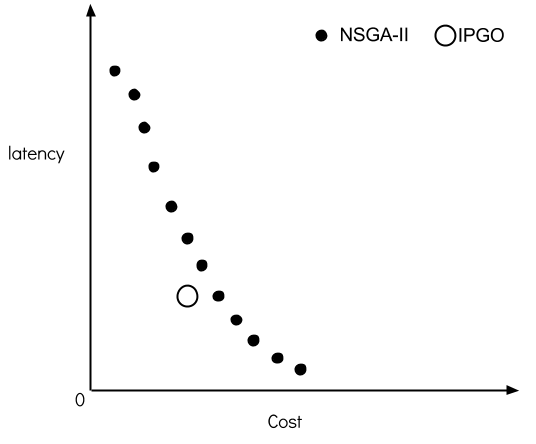
\includegraphics[width=\textwidth]{pics/3.png}
		\caption{}
	\end{subfigure}
	\begin{subfigure}[b]{0.4\textwidth}
		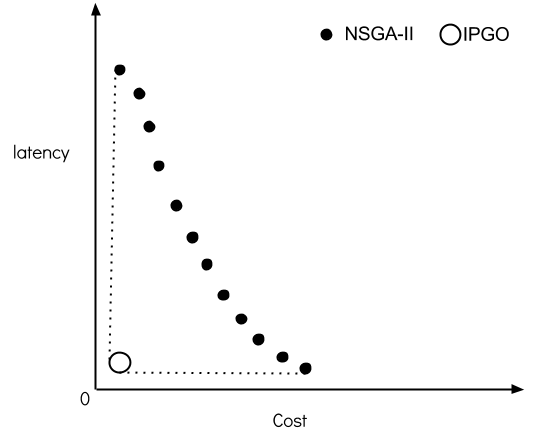
\includegraphics[width=\textwidth]{pics/4.png}
		\caption{}
	\end{subfigure}
	\caption{Four cases of the relation between a ALA solution and a NSGA-II solution set of non-dominated solutions}\label{fig:Pareto}
\label{fig:Pareto}
\end{figure}

The relation between a single solution and a set of non-dominated solutions from NSGA-II can be classified into four cases as shown
in Figure \ref{fig:Pareto}. (a), the ALA solution is dominated by some solutions in NSGA-II solution set. In this case, we can
say that NSGA-II outperforms ALA since the inclusion of the ALA solution does not improve the quality of the NSGA-II solution set.
On the other hand, we can say that ALA outperforms NSGA-II in Figure \ref{fig:Pareto} (d) Since the ALA solution dominates all
solutions in the NSGA-II solution set. In Figure \ref{fig:Pareto} (b), the ALA solution is non-dominated solution in the NSGA-II 
solution set. While the inclusion of the ALA solution somewhat improves the quality of the NSGA-II solution set, we cannot say that
ALA outperforms NSGA-II since the ALA solution dominates no NSGA-II solutions. We may intuitively say that NSGA-II outperforms
ALA in the case of Figure \ref{fig:Pareto} (b).

It is difficult to say which is better between ALA and NSGA-II in (c) where ALA solution dominates some NSGA-II solutions. If we
use performance measures that are strongly related to the convergence of solutions, ALA maybe evaluated as being better than
NSGA-II. On the contrary, if we related strongly to the diversity of solutions, NSGA-II may be evaluated as being better than ALA.



Parameter settings for application of NSGA-II are shown in Table \ref{table:para}. The terminal condition is that the 
population has evolved 50th generation.

\begin{table}[H]
\caption{NSGA-II Parameters}
\begin{center}
	\begin{tabular}{ | l | l | l | 1 | 1 |p{2cm} |}
		\hline
		Population & Generation & Tour Size & Crossover Rate & Mutation Rate \\ \hline
		50& 50 & 10 & 0.8 & 0.2 \\ \hline
	\end{tabular}
	\label{table:para}

\end{center}
\end{table}


\subsection{ALA}

Much research has been devoted to develop efficient heuristic algorithm to solve location-allocation problem. Two of the predominant
greedy construction heuristics are the ADD and DROP \cite{Sun} methods, which build solutions from scratch. 
An important greedy improvement heuristic is the Alternate Location-Allocation method which builds on an existing solution. 
The ADD procedure starts with all facilities closed and locates a facility that gives the greatest savings at each step and 
iterates through all potential locations until no further savings can be made. In contrast, DROP opens all facilities and removes a 
location that gives the greatest savings at each step and tries to find optimal or near optimum solutions at the end of the 
iterative procedure. ALA builds upon ADD and DROP methods. In order to solve multi-objective problem, ALA first uses Integer programming
to solve the problem in terms of cost.
		

\begin{equation}
     \begin{align}
       \mbox{Minimize } & \sum\limits_{s \in S} \sum\limits_{j \in J} C_{sj} \times A_{sj} \\
       \mbox{Subject to} & \\
	        & \sum\limits_{s \in S} A_{sj} \geq 1 \\
	        & \sum\limits_{s \in S} \sum\limits_{j \in J} C_{sj} \times A_{sj} \leq CostLimitation \\
     \end{align}
\end{equation}

Once a minimum cost solution is found, the solution set will be passed to the ADD procedure to serve as an initial solution for 
further improvement on Network latency. The ADD procedure as follows:
\begin{itemize}
	\item Evaluate network latency fitness of the initial solution.
	\item Starts a facility then evaluate with network latency fitness function. If the network latency fitness decreased as well as 
		the cost fitness does not exceed the cost constraint. The solution is kept.
	\item If there is no location could be choose, terminate the procedure.
\end{itemize}


\section{Experimental results}
\subsection{Efficiency comparison}

\begin{table}[!htb]
	\caption{Efficiency Test}
\begin{minipage}{.5\linewidth}
	\caption{Sufficient condition}
	\centering
	\begin{tabular}{ | l | l |p{2cm} |}
		\hline
		Matrix Size & GA time(s) &ALA time(s)\\ \hline
		$3 \times 3$  & 1.7 & 0.002\\ \hline
		$5 \times 5$  & 2.1 & 0.007\\ \hline
		$10 \times 10$ &3.775 & 0.11\\ \hline
		$15 \times 15$  & 6.355 & 0.64\\ \hline
	\end{tabular}
	\end{minipage}
	\label{table:sufficient}
%\end{center}
%\end{table}
%\begin{table}
%\begin{center}
\begin{minipage}{.5\linewidth}
	\caption{Good condition}
	\begin{tabular}{ | l | l |p{2cm} |}
		\hline
		Matrix Size & GA time(s) & ALA time(s)\\ \hline
		$3 \times 3$  & 1.71 & 0.003\\ \hline
		$5 \times 5$  & 2.07 & 0.01 \\ \hline
		$10 \times 10$ &3.6 & 0.11\\ \hline
		$15 \times 15$  & 6.26 & 0.6\\ \hline
	\end{tabular}
	\end{minipage}
	\label{table:good}
%\end{center}
%\begin{center}
\begin{minipage}{.5\linewidth}
	\caption{Poor condition}
	\begin{tabular}{ | l | l |p{2cm} |}
		\hline
		Matrix Size & GA time(s) & ALA time(s)\\ \hline
		$3 \times 3$  & 1.89 & 0.004\\ \hline
		$5 \times 5$  & 2.3 & 0.01 \\ \hline
		$10 \times 10$ &4.08 & 0.11\\ \hline
		$15 \times 15$  & 8.67 & 0.57\\ \hline
	\end{tabular}
	\end{minipage}
	\label{table:poor}
%\end{center}
%\begin{center}
\begin{minipage}{.5\linewidth}
	\caption{Minimum condition}
	\begin{tabular}{ | l | l |p{2cm} |}
		\hline
		Matrix Size & GA time(s) & ALA time(s)\\ \hline
		$3 \times 3$  & 1.88 & 0.003\\ \hline
		$5 \times 5$  & 2.67 & 0.01 \\ \hline
		$10 \times 10$ &6.06 & 0.11\\ \hline
		$15 \times 15$  & 15.4 & 0.6\\ \hline
	\end{tabular}
	\end{minipage}
	\label{table:minimum}
%\end{center}
\end{table}

As the experimental results show, in terms of the average run time, ALA is clearly better than NSGA-II. 
There are two main reasons: firstly, NSGA-II's run time is largely depend on the generation setting.
Second, repeat evaluation of chromosome is the decisive factor of time consuming. Although, the modified
NSGA-II tries to avoid unnecessary evaluation by employing the idea of memory pool, the improvement is limited. 

It is worth nothing that in sufficient condition and good condition, both algorithm's run time remain stable. The run time starts
increasing under poor condition and minimum condition with NSGA-II. In particular, the run time for $15 \times 15$ matrix under 
minimum condition is more than twice as under conditions.  The reason is that, in the constraint check process, 
If the children exceed the cost constraint, 
the repair operator will iteratively close facilities until it satisfied the cost limitation or minimum facility number is achieved. 
If the cost constraint is set too low, the number of iteration in the repair 
processes will reach a maximum number. Therefore, the time consuming increases largely.


\subsection{Effective comparison}
\label{sec:comparison}
\begin{figure}[H]
	\centering
	\begin{subfigure}[b]{0.4\textwidth}
		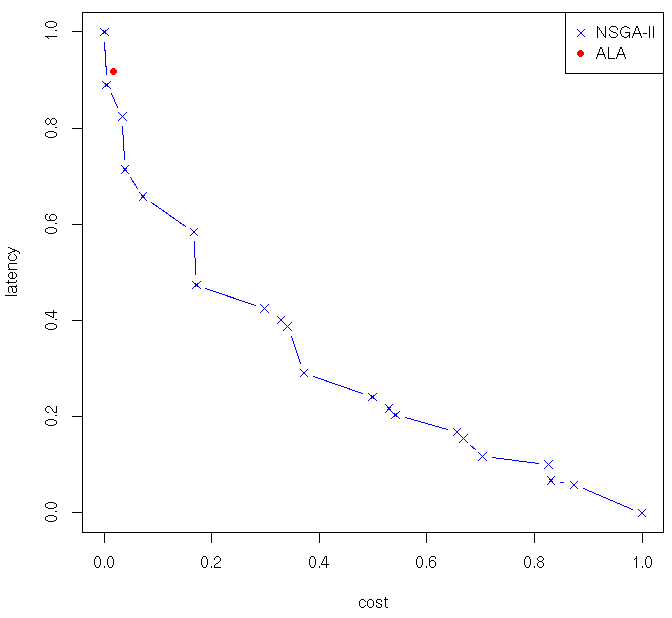
\includegraphics[width=\textwidth]{pics/105.png}
		\caption{$3 \times 3$}
		\label{fig:3_by_3}
	\end{subfigure}%
	\begin{subfigure}[b]{0.4\textwidth}
		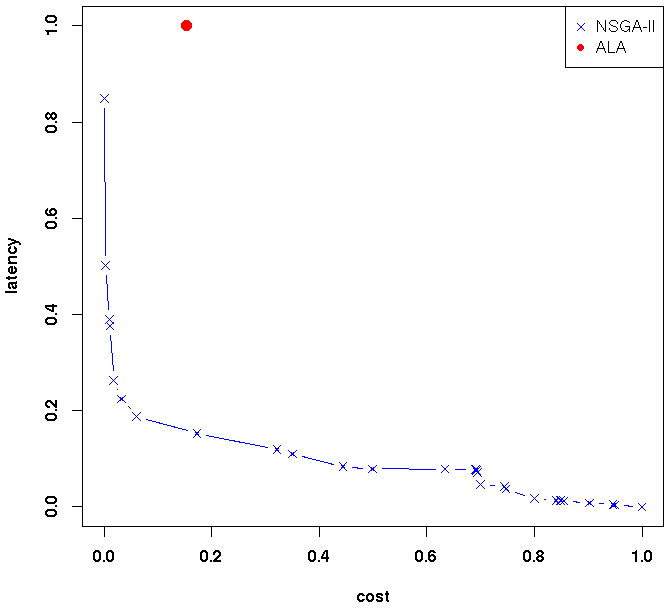
\includegraphics[width=\textwidth]{pics/107.png}
		\caption{$5 \times 5$}
		\label{fig:5_by_by_suff}
	\end{subfigure}


	\begin{subfigure}[b]{0.4\textwidth}
		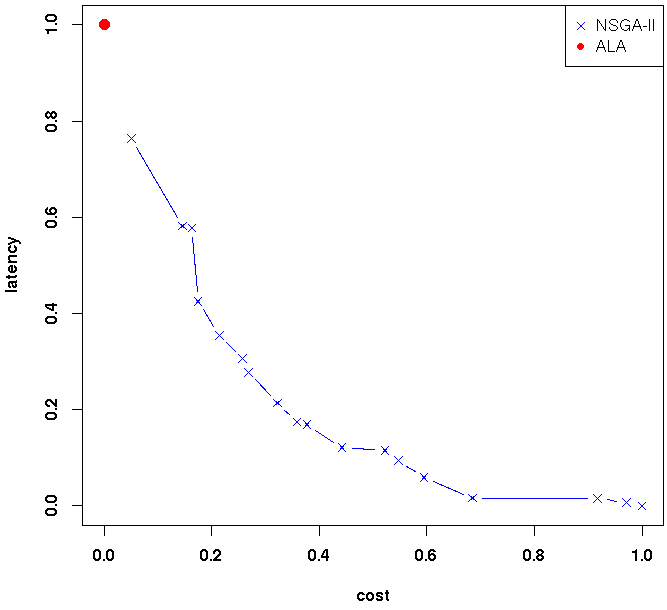
\includegraphics[width=\textwidth]{pics/111.png}
		\caption{$10 \times 10$}
		\label{fig:poor}
	\end{subfigure}
	\begin{subfigure}[b]{0.4\textwidth}
		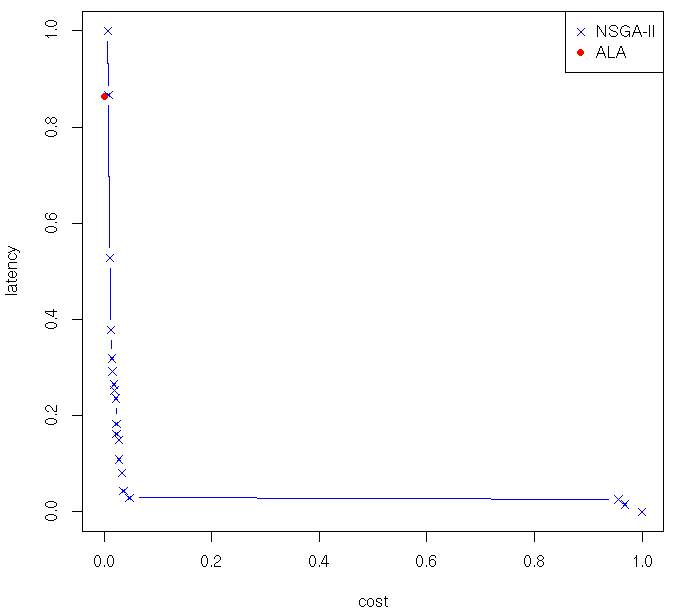
\includegraphics[width=\textwidth]{pics/112.png}
		\caption{$15 \times 15$}
		\label{fig:minimum}
	\end{subfigure}

	\caption{}\label{fig:condition}
\end{figure}


\section{Conclusion}
In this paper, we presented a modified NSGA-II for web service location allocation problem. Our approach utilizes a memory pool so that
greatly reduces the evaluation time while the diversity of the population gradually decreases. We have conducted a full experimental evaluation using the public WS-DREAM dataset to compare our approach to Alternate Location Allocation algorithm. 
The experimental results shows the modified is effective to provide a near-optima solutions for the web service location-allocation problem.

\bibliographystyle{apalike}
\bibliography{ecjsample}


\end{document}
